Article: ACLAC: An approach for adaptive closed-loop anesthesia control

\begin{abstract}
In current practice, to control the anesthetic process, the
anesthetist delivers drugs according to the surgery procedure and
% which the patient is undergoing
% , to the patient characteristics, and to the current patient state.
to the current patient characteristics and state.
%
This is an open-loop procedure requiring an active participation of
the medical expert.
%
We propose an adaptive closed-loop controller for the regulation of
hypnosis for patients undergoing general anesthesia.
%
One of the main problems arising when designing such a controller is
related to the intra- and inter-patient variability.
%
We employ a simple regression model to make prediction of patient's
response and to compute the adequate doses of propofol to keep the
patient in the specified Bispectral Index target.
%
To make our model adaptive, we continuously monitor the patient
behavior and detect changes in patient response to update the
identification model.
%
Experimental evaluation on real patients data shows that we can
effectively detect change points. Simulation of the adaptive
closed-loop control with the change detection mechanism also suggests
that the use of the adaptation mechanism improves the control. 
%and can be investigated further in the hospital settings.
\end{abstract}
%-------------------------------------------------------------------------
\section{Introduction}
The main variables appearing in anesthesia are hypnosis, analgesia and
muscular relaxation. Hypnosis refers to the level of unconsciousness
of the patient. Analgesia is related to the level of insensibility to
pain. And muscular relaxation is also a variable of interest to avoid
movements during the surgical procedure and to make easier access to
patient’s organs.

In the anesthetic process, the clinician must guarantee an adequate level for these three variables.
% ... CHANGED TO:
% To achieve this, the anesthetist delivers drugs according to the surgery procedure to which the patient is undergoing,
% to the patient characteristics, and to the current patient state.
% ... TO:
% To achieve this, the anesthetist delivers drugs according to the surgery procedure, to the patient characteristics and state.
% %
% Traditionally the anesthetist starts with the infusion of these drugs according to well established protocols and then
% modifies the infusion depending on the clinical signs observed during the procedure.
Traditionally the anesthetist starts with the infusion of the drugs according to well established protocols and then
modifies the infusion depending on the patient characteristics and state.
%
%... Compressed:
% As can be observed this is an open-loop procedure, and
% only appears through the clinical observations of the medical expert.
%... To:
As can be observed this is an open-loop procedure.

During last years the introduction of closed-loop methodologies in
this field has been a matter of study and some closed-loop strategies
have been reported with real patients in the operating theater. These
approaches propose to consider both signal-based
~\cite{mendez_adaptive_2009,reboso_design_2012} and model-based
control schemes ~\cite{liu_closed_loop_2011, nino_epsac_controlled_2009}.
%
Most of them are focused in the regulation of the hypnosis level of
the patients once they become unconscious.
% COMPRESSED: (DELETED)
% The regulation of the
% analgesia level is quite more difficult due to the non-availability of
% a reliable index to measure the analgesic state.
%
% DELETED: "However, "
The hypnosis level can be measured through an index extracted
from the electroencephalogram (EEG). This variable is called
Bispectral Index (BIS)~\cite{bis} and is well correlated with the
level of unconsciousness. %related work on this is missing, i.e. we need to position wrt this existing work

We propose an adaptive closed-loop controller for the regulation of
hypnosis for patients undergoing general anesthesia and
% COMPRESSED (REMOVED): : because the same words are used further in second section - The problem of anesthesia control.
% One of the main problems arising when designing such a controller is
% related to the intra- and inter-patient variability.
% DELETED: "We"
employ a simple regression model to make prediction of patient's
response and to compute the adequate doses of propofol to keep the
% DELETED: (Bispectral Index) ADDED: "value"
patient in the specified BIS value target.
%
To make our model adaptive, we continuously monitor the patient
behavior and detect changes in patient response to update the
identification model.

The rest of the paper is organized as follows.
% NOT CHANGED
In Section~2 we introduce the problem of anesthesia control and emphasize the challenges to be addressed.
% TO:
%In Section~2 we introduce the problem of anesthesia control.
%
In Section~3 we present ACLAC -- our approach for adaptive closed-loop
anesthesia control that has a change detection mechanism built into
it. In Section~4 we discuss the results of the experimental study
including the simulation of the closed-loop anesthesia control on the
simulated data and the performance of the change detection on the real
data collected from ten different patients during in the surgery room.
Experimental evaluation on real patients data shows that we can
effectively detect change points. Simulation of the adaptive
closed-loop control with the change detection mechanism also suggests
that the adaptation mechanism is adequate and can be investigated
further in the hospital settings. Section~5 concludes with the
discussion of the limitation and future work.

\section{The problem of anesthesia control}
This work focuses on the regulation of hypnosis for patients undergoing general anesthesia.
% ADDED:
As a feedback variable for a close-loop control of a hypnosis we use the BIS signal.
%
In particular we considered a BIS target of 50~\cite{luginbuhl,rampil}.
%
The hypnotic drug used is intravenous propofol.
%
The control objective is to maintain the BIS in 50 rejecting the disturbances affecting
the patient during the procedure: surgical stimuli, blood loss, incisions, etc.

%
BIS variable is adimensional and varies between 100 (awake state) and 0 (no electrical brain activity).
%
% Compressed(removed):
% Different bands can be defined according to the state of the patient.
%
% Compressed:
% Thus, the values of BIS between 60 and 40 define the band for general
% anesthesia.
% To:
The values between 60 and 40 define the band for general anesthesia.
%
% Compressed:
% The availability of the BIS signal make it feasible to propose a
% close-loop control for hypnosis using this variable as the feedback
% variable.
% To:
% We propose a close-loop control for hypnosis using this variable as the feedback variable.

% CHANGED:
% One of the main problems arising when designing the controller is
% related with the patient variability.
% TO:
One of the main problems arising when designing the controller is
the patient variability.
%
We can distinguish both inter-patient and intra-patient
variability. Inter-patient refers to the variability appearing in the
response to the drug between different patients.
%
% COMPRESSED:
% And intra-patient variability appears because during surgery the
% response of the same patient along the procedure is changing with
% time.
% TO:
And intra-patient variability appears because of change in the
response during surgery of the same patient along the procedure.

% Removed: "Thus, one.."
An important specification that the closed-loop controller must
satisfy is the robustness to this variability.
%
From the control engineering point of view, two different approaches
can be used.
%
The basis of robust control is to design a fixed controller that
offers satisfactory performance even if the patient response
changes.
%
A different option is the use of adaptive controllers that includes
adaptation mechanism to change in response to changes in the patient.

In this work, we propose a predictive adaptive controller that
continuously monitors the patient behavior, propose a model to make
prediction of his response and computes the adequate doses of propofol
to keep the patient in the specified BIS target.

The sample time considered is 5 seconds. Although, according to
patient response, a bigger value can be considered, this sample time
is large enough to guarantee the applicability of the controller in
terms of computational burden.

\section{Approach}
Our approach consists of three main components: adaptive patient
modeling, control and change detection mechanisms that we describe in
the corresponding subsections.

\subsection{Adaptive modeling of hypnosis}
%As commented above, a predictive controller was designed using an adaptive patient model.
The common approach to model the patient dynamics to propofol infusion
is the use of compartmental models. %ref to compartmental models is missing
This approach considers different compartments interconnected and with
a given time constant. Drug is infused in the main compartment, and
from then is transferred to the other compartments until equilibrium
is reached between all the compartments. A common approach considers
four compartments (central, slow, fast and \textit{effect
  site})~\cite{schnider_influence_1998}.
%
The BIS variable can be obtained as a nonlinear function of the
concentration in the effect site compartment.

We use a linear approximation to this model using an Autoregressive
with exogenous input (ARX) model that computes the input signal at
sample instant $d$ as a function of the input and output values at
previous time instants. The computation of the model parameters is
done online by using a least squares minimization algorithm.
%
%   COMPRESSED(REMOVED):
%
Consider the following polynomials:
\[
A(z^{-1})=1+a_{1}z^{-1}+a_{2}z^{-2}+...+a_{na}z^{-na}
\]
\[
B(z^{-1})=b_{0}+b_{1}z^{-1}+b_{2}z^{-2}+...+b_{nb}z^{-nb}
\]
\noindent
% deleted: where $na$ and $nb$ are the degrees of the polynomials and $z^{-1}$ is the \textbf{delay operator}.
where ${na}$ is the number of previous \emph{outputs} and ${nb}$ is the
number of previous delayed by $n_{d}$ \emph{inputs} on which the
current output depends and $z^{-n}$ is the \emph{delay operator}
which is defined by $z^{-n}x(t)=x(t-n)$.  Then, the ARX model for the
BIS variable can be expressed as:
\[
A(z^{-1})BIS(t)=B(z^{-1})u(t-n_{d})+e(t)
\]
\noindent
% http://www.ncbi.nlm.nih.gov/pubmed/8695136
% variable-rate propofol infusion up to 0.15 mg/kg/min
where $BIS(t)$ is the $BIS$ value at $t$, $u(t)$ represents the propofol infusion rate in $mg/l/min$, $e(t)$ is the residual
error and $n_{d}$ is the input-output delay.
Thus, the model can be expressed as:
\begin{multline}
BIS(t)+ a_{1} BIS(t-1)+...+ a_{na} BIS(t-na) = \\
b_{0}u(t-n_{d})+ b_{1}u(t-n_{d}-1)+...+ b_{nb} u(t-n_{d}- n_{b})+e(t)
%\label{eq:model}
\end{multline}
% % Added:
% where $\pmb{na}$ is the number of previous \textbf{outputs} and $\pmb{nb}$ is the
% number of previous delayed by $\pmb{n_{d}}$ \textbf{inputs} on which the
% current output depends.
% %
% $BIS(t)$ is the $BIS$ value at $t$, $u(t)$ represents the  propofol infusion rate in $mg/l/min$, $e(t)$ is the residual error.
%
% COMPRESSED:
% The choice for $na$, $nb$ and $n_{d}$ was done using simulations.
% In this work we use $na=nb=4$ and $n_{d}=1$.
% TO (ADDED: "least squares algorithm"):
The estimation for $na=nb=4$ and $n_{d}=1$ was done using least squares algorithm during simulations.
%
% COMPRESSED (REMOVED): : The same appears earlier as: "The computation of the model parameters is done by using a least squares minimization algorithm."
% We use an online least squares algorithm to compute the A and B
% polynomials using past information of the process.
%
% COMPRESSED REMOVED "Thus.":
The model will adapt to the specific patient response and to eventual changes in its dynamics.
% not changesd TO:
% The model will adapt to the patient response and to changes in its dynamics.
%
Figure~\ref{fig:ARXmodel} shows the identification scheme used.

\begin{figure}[htb!]
\centering
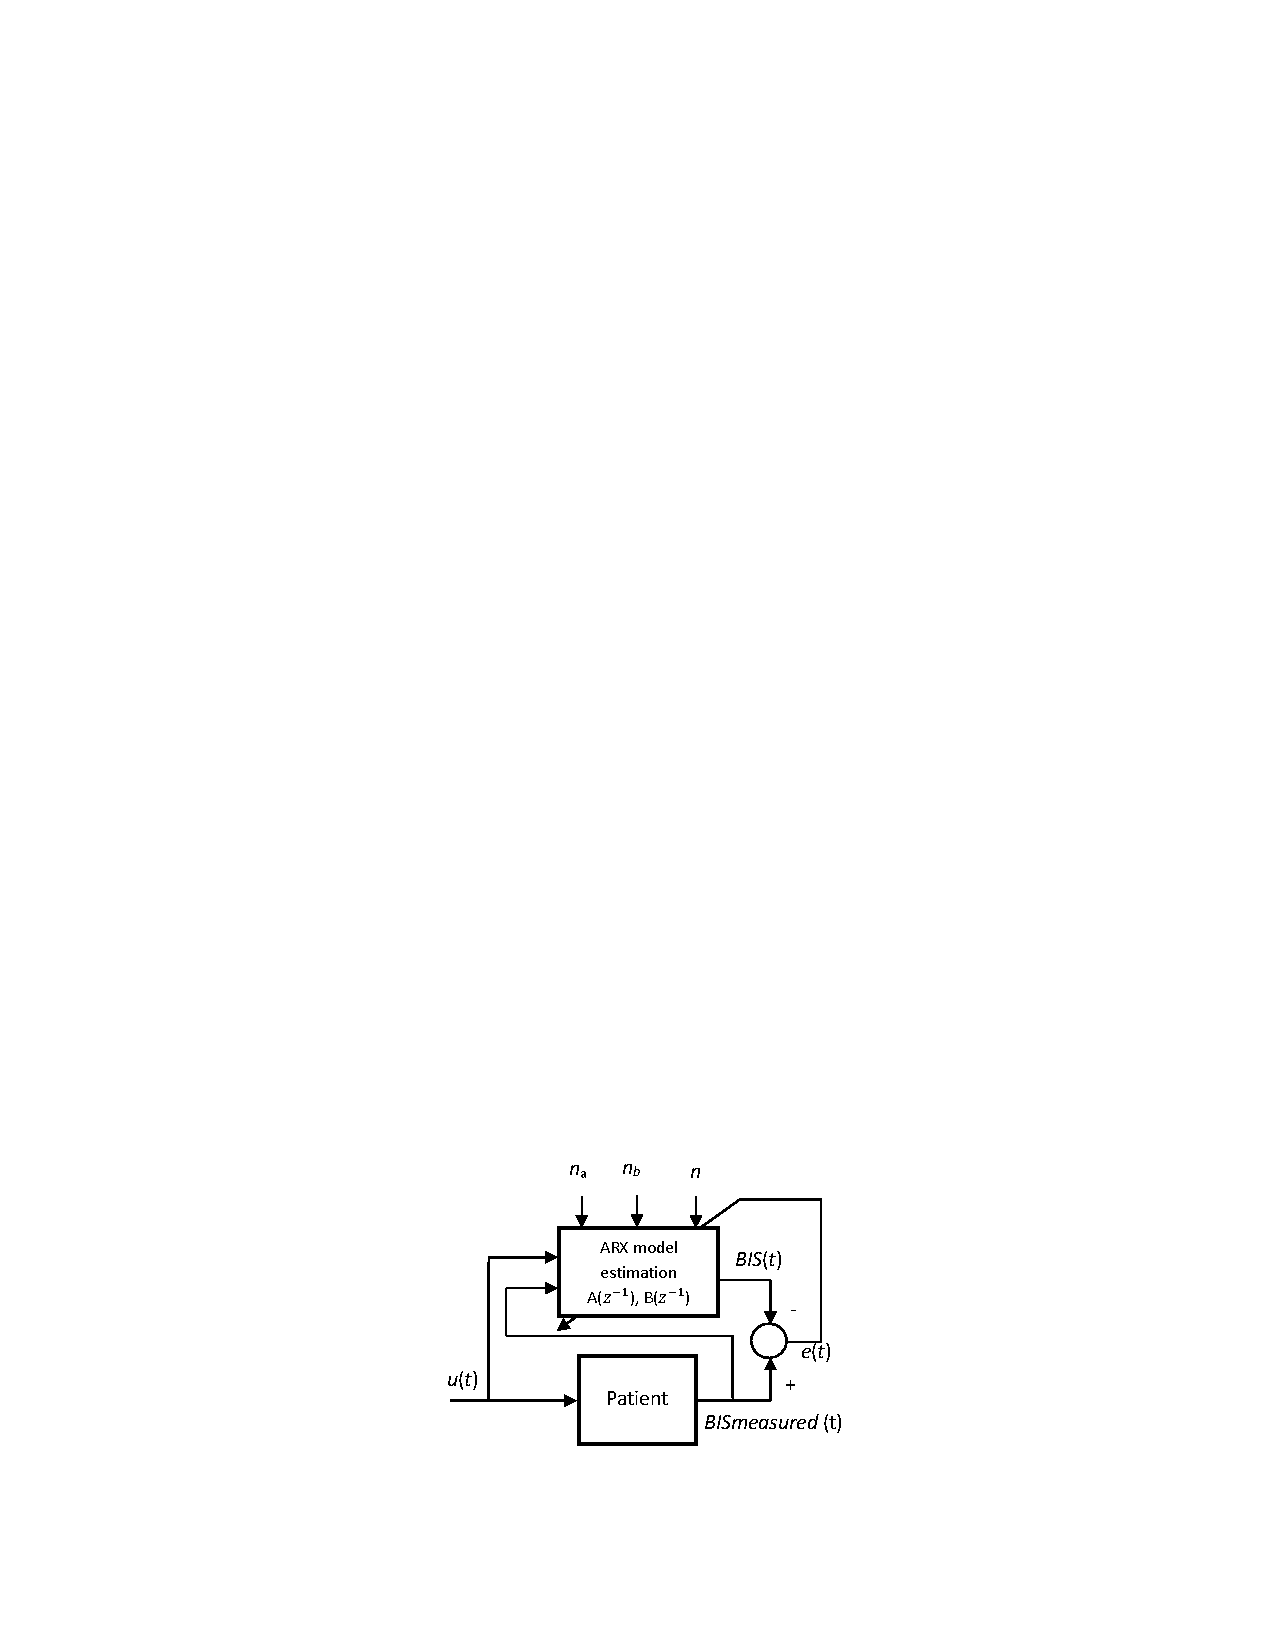
\includegraphics[width=0.4\textwidth]{./pics/aclac_paper/ARXmodel.pdf}
\caption{Patient model identification.} %scheme
\label{fig:ARXmodel}
\end{figure}

% CHANGED:
% The initial model chosen for the patient is a standard model obtained from the analysis of a set of real patient data.
% TO:
The initial model for the patient is estimated from the analysis of a set of real patient data.
%
After the initial training, the adaptation algorithm proposes a new
model based on real data of the patient. This model is regularly
updated along the time.

% CHANGED:
% One important issue to improve the accuracy of the model
% identification scheme is the availability of information of patient
% changes.
% TO:
% The availability of information of patient changes can improve the
% accuracy of the model identification scheme.
% CHANGED:
% This information would be used in the identification subsystem to make
% decisions about the relevance of the patient data used in the
% identification algorithm.
% TO: DELETED:""
% This information would be used in the identification subsystem to make
% decisions about the relevance of the patient data used in the identification algorithm
% CHANGED TO:
The availability of information of patient changes can improve the
accuracy of the model identification scheme which would be used to
% DELETED: identification
make decisions about the relevance of the patient data used in the algorithm.
% Thus, one contribution of this paper is the inclusion of a change
% % DELETED " eventual" from " eventual changes"
% detection algorithm to detect changes in patient response and use it to improve the identification performance.
% TO:
Thus, one contribution of this paper is the inclusion of a change
detection mechanism to detect changes in patient response.
%improve the identification performance. - mentioned in the previous sentence
%
% DELETED : "simply"
In ACLAC we disregard data preceding to a detected changepoint.
This way, the model update will only include information of the new dynamics of the patient.
%This scheme will improve the performance obtained with adaptive schemes based in fixed time window.

\subsection{Control approach}
The controller proposed to regulate the hypnosis of the patient is shown in Figure~\ref{fig:Controller}.
%
% COMPRESSED:
% As can be observed the model predictive controller(MPC) decides the adequate profofol infusion rate to be infused to the patient.
% TO:
The model predictive controller(MPC) decides the adequate profofol infusion rate to be infused to the patient.
%
The MPC uses a linear model for the predictions that is obtained from the model identification module.
%
% COMRESSED: : REMOVED - "As commented,"
The change detection algorithm provides information to the identification scheme that is used to determine the time-window of
past data used.
\begin{figure}[htb!]
\centering
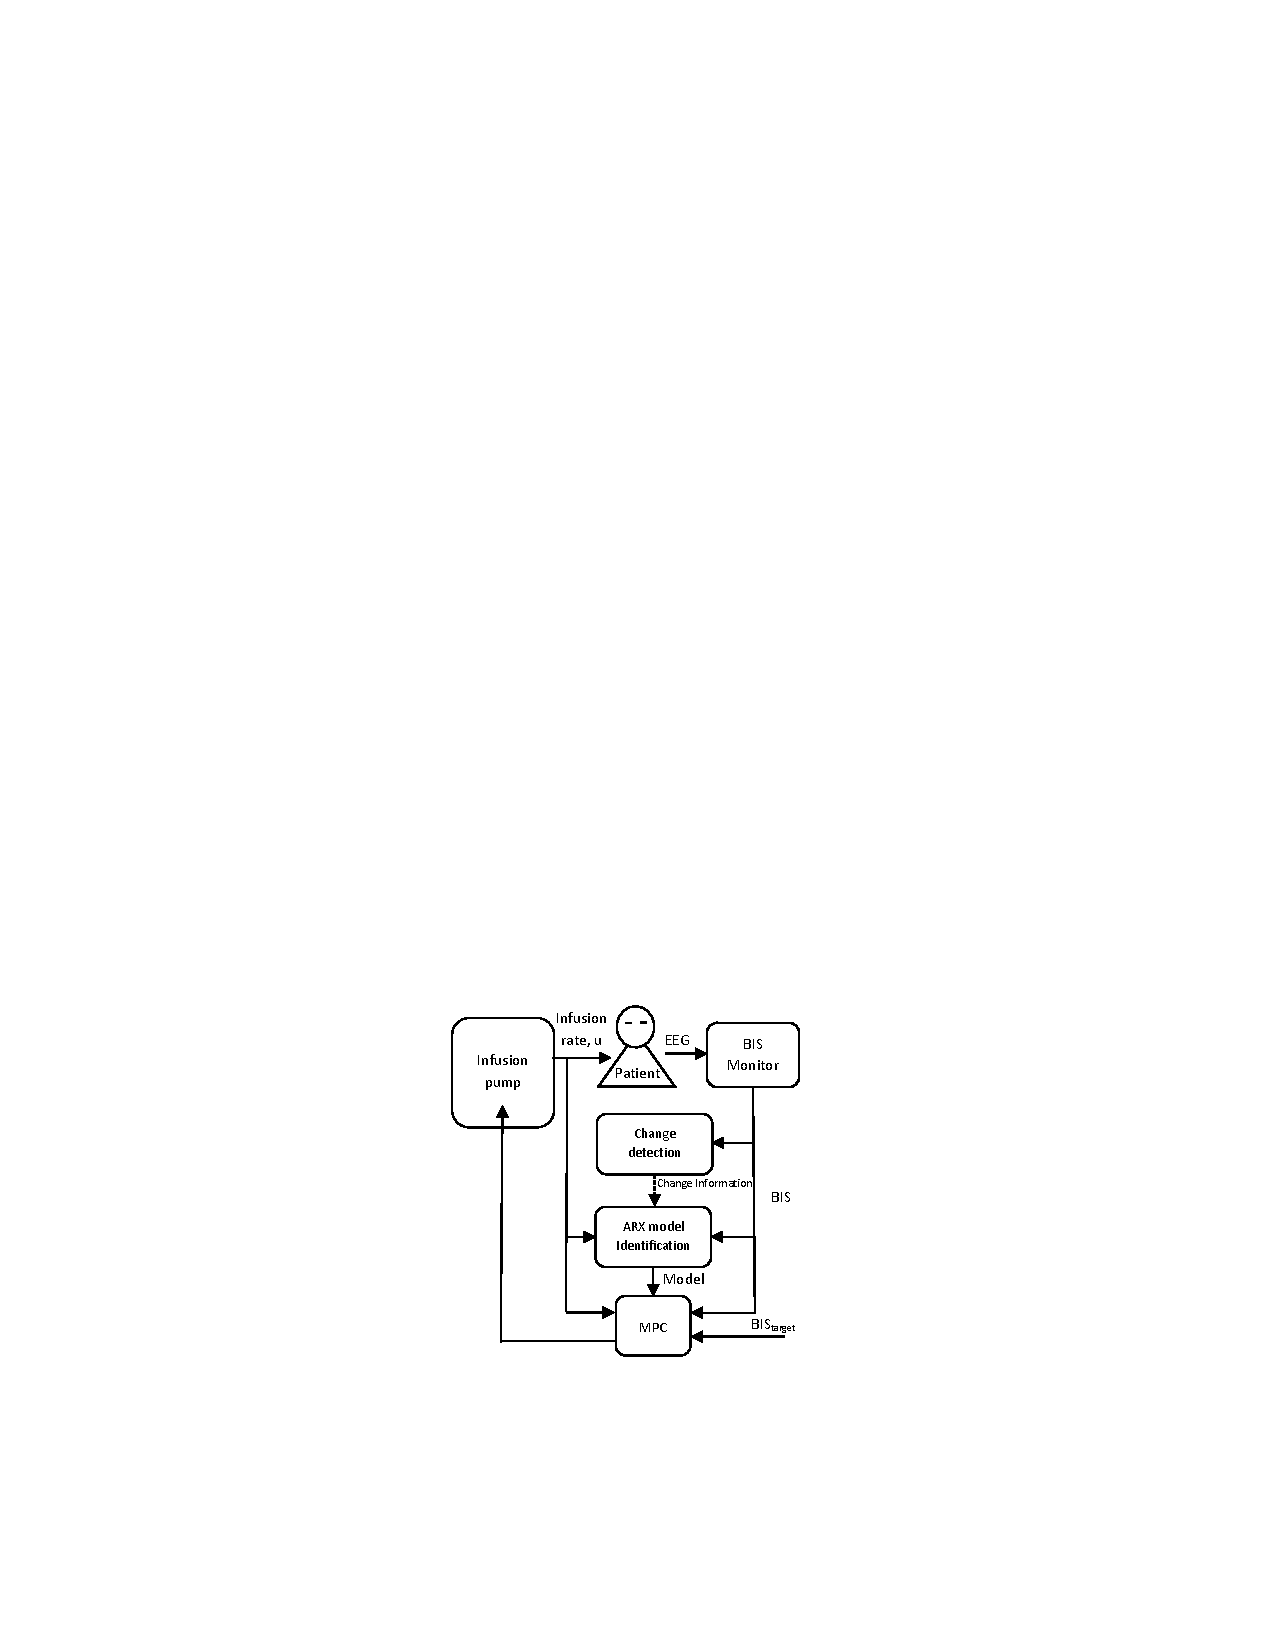
\includegraphics[width=0.40\textwidth]{./pics/aclac_paper/Controller.pdf}
\caption{Closed-loop control scheme using identification scheme with change detection.}
\label{fig:Controller}
\end{figure}
% Model predictive control
% CHANGE: "consists of" to "includes"
MPC controller includes an optimization process in which the best
future inputs are computed based on the minimization of a given
function costs. The cost function uses predictions obtained with the ARX model.
% CHANGE: DELETED: "provided by the identification subsystem."

The formulation of the problem can be done as follows~\cite{Bordons}:
%\begin{equation}
\begin{multline}
\min\limits_{u(k|k),...,u(k+p-1|k)} \sum_{i=1}^{p} w_{i}(BIS(k+i|k)-BIS_{\textit{target}})^2 \\
+ \sum_{i=1}^{c}r_{i}\Delta u (k+i-1|k)^2
\end{multline}
subject to % equation~\ref{eq:model}.
\begin{multline}
%BIS(t)+a_{1}BIS(t-1)+...+a_{na}BIS(t-na) = \\
% b_{0}u(t-n_{k})+b_{1}u(t-n_{k}-1)+...+b_{nb}u(t-n_{k}-n_{b})
BIS(t)+a_{1}BIS(t-1)+...+a_{na}BIS(t-na) = \\
 b_{0}u(t-n_{d})+b_{1}u(t-n_{d}-1)+...+b_{nb}u(t-n_{d}-n_{b})
\end{multline}
\begin{multline}
BIS_{max} \ge BIS(k+i|k) \ge BIS_{min}, i=1,...,p \\
u_{max} \ge u(k+i-1|k) \ge u_{min}, i=1,..,c \\
\Delta u_{max} \ge \Delta u(k+i-1|k) \ge -\Delta u_{max}, i=1,..,c
\end{multline}
\noindent
where $k$ is the current time instant, $p$ and $c<p$ are the sizes of
the prediction horizon and control horizon respectively,
$BIS_{target}$ is the target for the $BIS$, and $u(k+i-1|k)$,
$i=1,...,p$, is the set of future input values, where
\begin{multline}
u(k+i|k)=u(k+c-1|k), i=c,...,p-1 \\
\Delta u(k+i-1|k)=u(k+i-1|k)-u(k+i-2|k)
\end{multline}
The optimization problem is solved at time instant $k$. Under this
approach, the control law for $u(k|k)$ is obtained by solving a
quadratic programming problem. The optimal input $u(k)=u_{opt}(k|k)$
is applied to the plant. This process is repeated in subsequent times
$k+1, k+2$, etc.  Thus the new control law $u(k +1|k +1)$ may be
different from the control signal calculated above. This principle is
called moving horizon strategy.
%----------------------------------------------------------------------%
%-------------------- CHANGE DETECTION METHOD -------------------------%
%----------------------------------------------------------------------%
\subsection{Change detection method}
\label{sec:ChangeDetectionMechanism}
%
The term change point stands for a phenomenon when statistical
properties of a data stream change significantly over time.
%
In medical sensor data streams we can observe changes of different
types: change in the mean value, variance, autocorrelation, in the
seasonal and trend components, etc. Changes can be classified also
with respect to the rate of the change into abrupt and gradual
changes. These changes, strictly speaking, are happening almost
continuously (depending on the `scales' of the changes which we
% DELETED "And" from "And one of the problems"
consider). One of the problems is to define rules by which we can
determine whether change is significant and should be detected
% DELETED: "(alerted)"
or not.
%
Such rules can be constructed using state-of-the-art change detection
methods based on control charts, cumulative sum (CUSUM,~\cite{Cusum}),
heuristic (thresholding) approaches, two sliding windows statistic
monitoring (w.r.t.\ data or modeling error), likelihood and density
ratio estimation for two competitive models among others~\cite{Nikiforov}.

We are interested in detection of the change in the mean value because
a BIS target value is 50 and control limits are defined by horizontal
lines of values 40 and 60.
% % COMPRESSED: REMOVED
% %is the following true?
% The most natural method for our task of change detection in BIS signal
% seems to be control charts or CUSUM method. In that case there is a
% need to define part of the signal which is `in control' and after that
% we can calculate control limits and ARL (Average Run Length) and other
% initial parameters values. But because of patient's inter- and
% intra-variability control limits and target value can slightly change
% between different patients or along the procedure for one patient.

In the domain of depth of anesthesia monitoring the problem of change
detection has been studied recently~\cite{GamaDecisionSupportSystems}.
A Page-Hinkley test with a forgetting mechanism (PHT-FM) was proposed
in~\cite{GamaRealTimeAlg}. This method is
on-line, %(unlike one used in our approach, which should be considered as `pseudo' on-line)
but it needs threshold value tuning that maybe not easy to achieve in
our case when dealing with noisy data or presence of outliers. Also it
requires the availability of training data on which the models can be
tuned.

%say, what the actual requirements are, e.g. wrt running time
%is the following true? none of the following is justified here
For our purposes we need a method which satisfies the following
conditions: 1)~it is applicable in an on-line settings, 2)~it is able to
detect multiple change points, 3)~it should take into account all
detected change points and decide on-line which of them should be
dropped because of the change in the scales of the changes.

% CHANGED:
%The commonly used approach for a single change point in a fixed interval is to perform likelihood ratio statistical hypothesis test.
% TO:
The commonly used approach for a single change point in a fixed interval is to perform likelihood ratio test.
%
In case of a single change point the null hypothesis $H_{0}$ is no
change point, alternative hypothesis $H_{1}$ is a single change point
at the moment of time $\tau$.
%
In other words, likelihood ratio test compares the fit of two
models, one of which is a special case of the other.
%
Given sequence of data $y_{1:n}=(y_{1},...,y_{n})$, it is said that
change point occurs at the moment of time $\tau$, such that the
statistical properties of $(y_{1},...,y_{\tau})$ and
$(y_{\tau+1},...,y_{n})$ are different accordingly to the chosen rules.
%
Twice the negative log-likelihood ratio function is used as a test
statistic to decide whether the change has occurred.
\begin{equation}
%ML(\tau_{1})=\log p(y_{1:\tau_{1}}| \hat{\theta_{1}}) + \log p(y_{(\tau_{1}+1):n}| \hat{\theta_{1}})
L(\tau)= \sum_{i=1}^{\tau}  \log p( y_{i}|\hat{\theta_{0}} ) + \sum_{i=\tau+1}^{n} \log p(y_{i}| \hat{\theta_{1}})
\end{equation}
\noindent
where $\hat{\theta}=(\mu, \sigma)$ is the maximum likelihood estimate of the parameters from likelihood function:
\[
\log p (y_{1:n}|\theta) =  -\frac{n}{2} \log(2 \pi) - \frac{n}{2} \log(\sigma^2) - \frac{1}{2\sigma^2} \sum_{i=1}^{n}(y_{i}-\mu)^2
\]
The test statistic is
\begin{equation}
\label{eq:gamma}
\lambda=C(y_{1:n}) = 2[\displaystyle \max_{\tau} L(\tau) - \sum_{i=1}^{n} \log p(y_{i}|\hat{\theta})]
\end{equation}
\noindent
%
where $\max\limits_{\tau} L(\tau)$ is the maximum log-likelihood
value under the alternative hypothesis.  The null hypothesis is
rejected if $\lambda > c$ where $c$ is selected threshold~\cite{KillickRpackage}.

In case of multiple change points the following function should be minimised:
\begin{equation}
\label{eq:optimal_partitioning}
\sum_{i=1}^{m+1}[C(y_{(\tau_{i-1}+1):\tau_{i}})] + \beta
\end{equation}
\noindent
where $m$ is the number of change points, $C$ is the twice negative
log likelihood cost function(Eq.~\ref{eq:gamma}) and $\beta$ is a
penalty term~\cite{KillickOptimalDetection} to prevent overfitting.
Value of $\beta$ was tuned during experiments.
%
%The term `changepoint' mostly refers to the situations when change is detected given fixed amount of data (moving interval during on-line monitoring) while the term `time-series segmentation' refers to algorithms which deal with a whole data set. During the segmentation data is split in such a way that we obtain the maximum difference (measured by the cost function) between emerged segments.
%
The combination of on-line monitoring algorithms and time-series segmentation methods is a promising approach for BIS monitoring because we often do not know in advance scales of the changes. Therefore, we have to perform analysis offline over detected points in order to discard (or keep) some of them if it is necessary.
%
For multiple change points detection we use PELT method
~\cite{KillickOptimalDetection}, which is based on dynamic programming
optimal partitioning algorithm proposed in~\cite{Barnes}.
%
Optimal partitioning algorithm performs recursive process that minimise function(Eq.~\ref{eq:optimal_partitioning}).
%
PELT method contains the pruning step within the dynamic
% DELETED: "significantly"
program which reduces computational cost of the method.
%
Comprehensive overview of the methods and description of the optimal
partitioning and PELT algorithms with pseudo-codes can be found in
~\cite{KillickOptimalDetection, KillickRpackage}.
%...........................................................%
%... EXPERIMENTAL STUDY / EVALUATION OF CHANGE DETECTION ...%
%...........................................................%
\section{Experimental study}
The validation of the proposed algorithm is done using real data
obtained from 10 patients undergoing general anesthesia. Patients are non
premedicated of ASA class I-II, scheduled for gynecological or
abdominal surgery with an estimated duration more than 30 minutes. A
laptop PC records both the BIS values and the infusion rate using
RS-232 links. The measurement of the BIS variable is done with a
{BIS-XP\texttrademark} monitor (Aspect Medical System) connected using
a RS-232 link and using four $ZipPrep^{\textregistered}$ electrodes. A
Graseby $3500^{\textregistered}$ infusion pump (Graseby Medical Ltd) with
propofol 1\% is the actuation system and was also connected via RS232
port to the PC. Sample time was 5 seconds.
% CHANGED:
% The data collected included both the induction phase and the maintenance phase.
% TO:
The data collected included both the induction and the maintenance phase.
%
In the induction phase a bolus dose is applied to take the patient
rapidly to the target area. In the maintenance phase the infusion rate
is calculated to keep the patient in the target BIS.

\subsection{Evaluation of change detection}
Change points for two signals are shown in
Figures~\ref{fig:ChangeDetection1}~and~\ref{fig:ChangeDetection2} (vertical dashed red lines).
%
% Totally, we considered signals from ten patients. % Mentioned at the beginning of section Experimental study.
%
The horizontal lines depict the target value and the general
anesthesia band.  In Figure~\ref{fig:ChangeDetection1} we can see that
the detected change points divide observations into four stages. The
first stage is short and has a high variance, but BIS is the in
control limits. In the second stage BIS is between the target value
and the upper limit. In the third stage BIS is below the target value,
but above the lower limit. In the fourth stage BIS is fluctuating
around the target value.  In Figure~\ref{fig:ChangeDetection1} we can
see that all out of limits periods are detected by the change
detection mechanism.

The detected change points represent 'changes' in a statistical
sense. It is described in subsection~\ref{sec:ChangeDetectionMechanism}.
Visual inspection of changes is difficult even for the domain experts.
Having no exact points on the BIS signals denoting ground truth
changes makes its hard to assess accuracy of detection in a
quantitative way.
% ?:
%Change points determine moments when regression model is updated using only relevant time windows.
\begin{figure}[htb!]
\centering
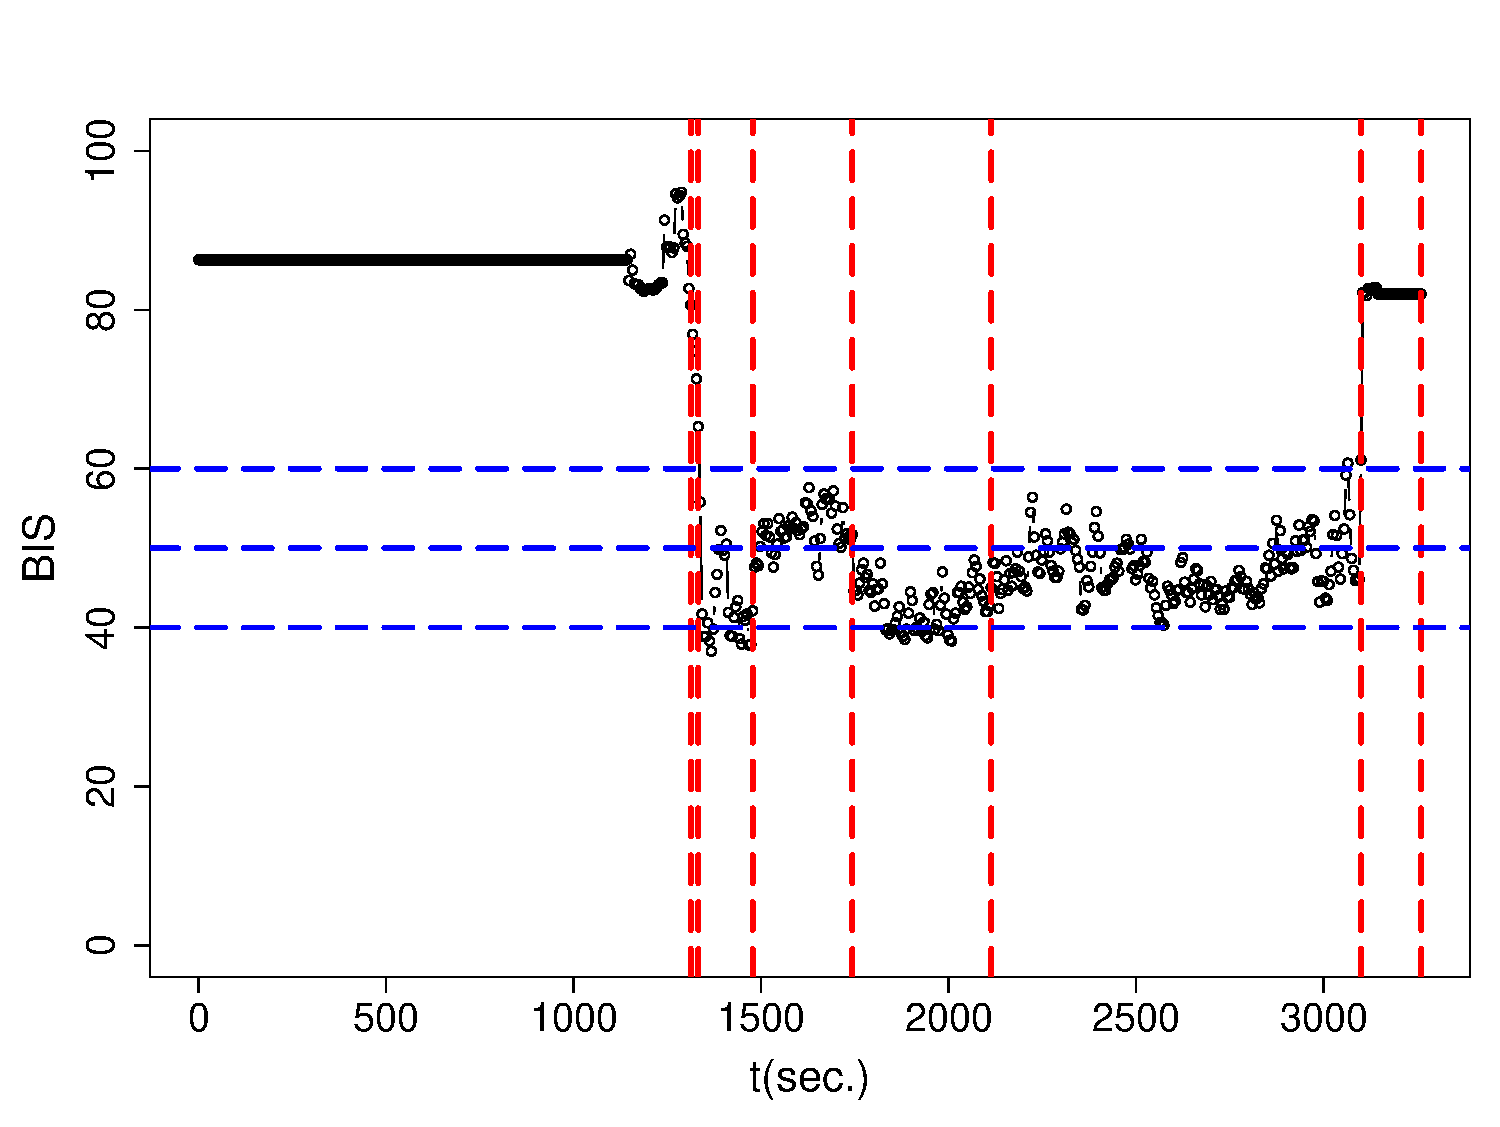
\includegraphics[width=0.40\textwidth]{./pics/aclac_paper/ChangeDetectionImage4.pdf}
\caption{Four stages detected in BIS.}
\label{fig:ChangeDetection1}
% COMPRESS:
%\end{figure}
%\begin{figure}[htb!]
\centering
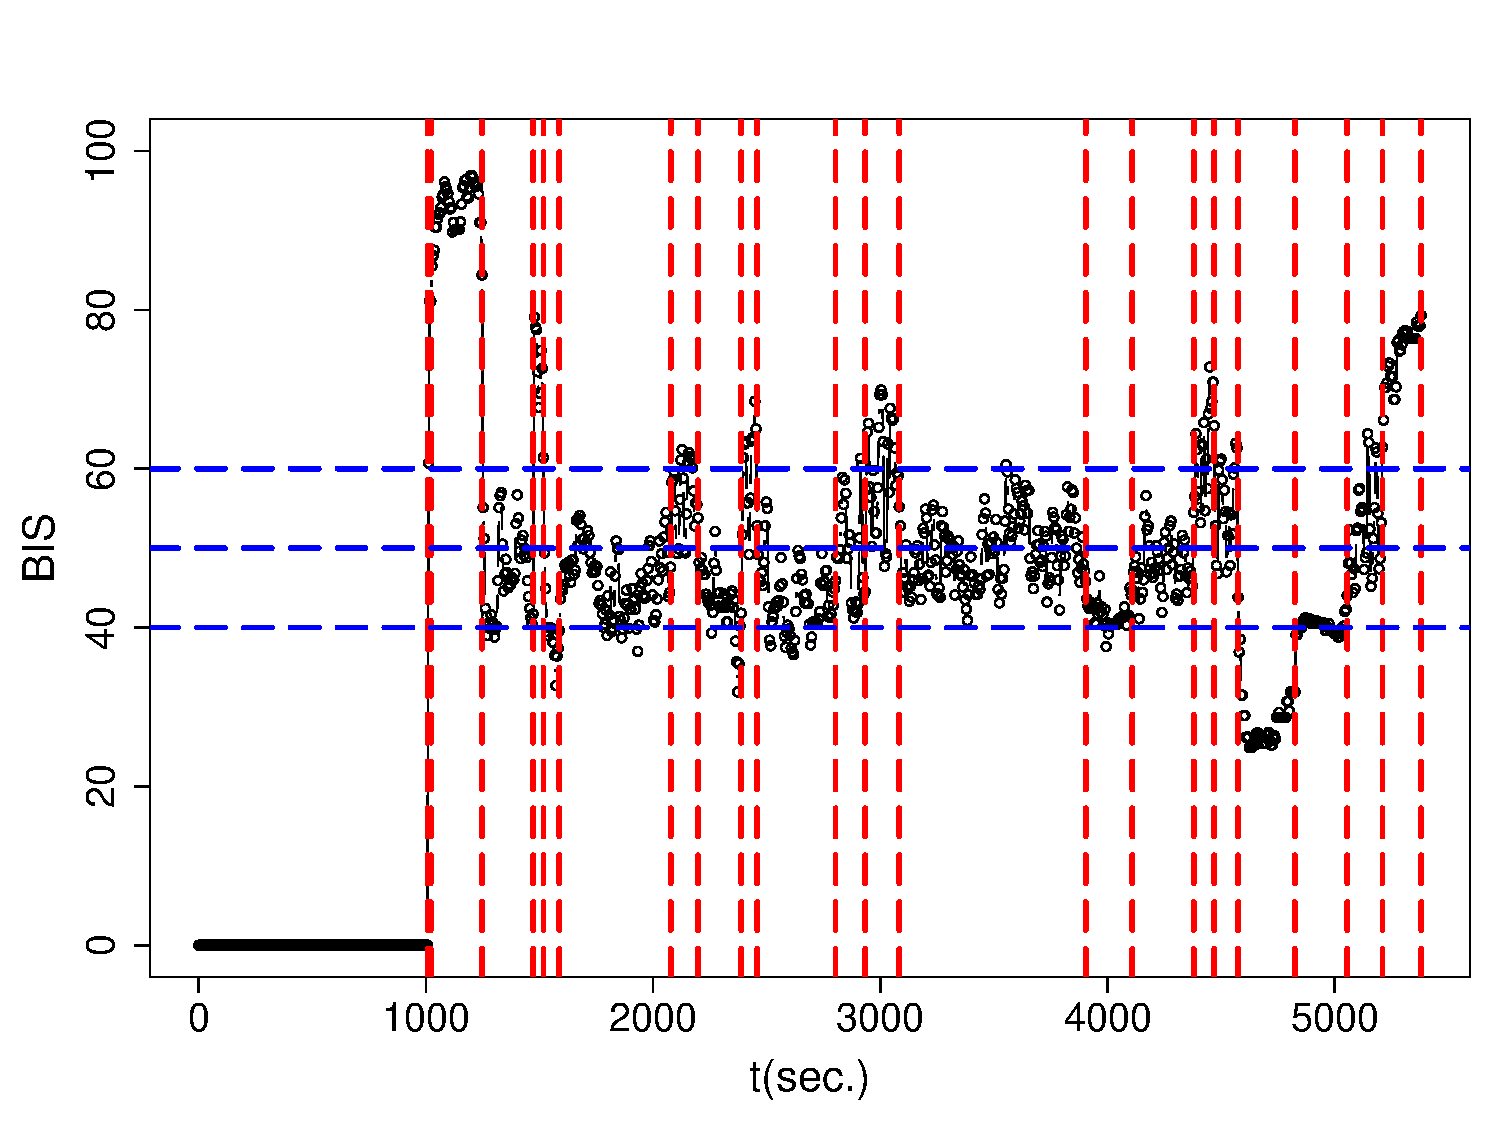
\includegraphics[width=0.40\textwidth]{./pics/aclac_paper/ChangeDetectionImage6.pdf}
%\caption{Change detection in BIS with high variance.}
\caption{Case of BIS with high variance.}
\label{fig:ChangeDetection2}
\end{figure}
%...........................................................%
%........................ LIMITATIONS ......................%
%...........................................................%
%\subsection{Limitations of change detection mechanism}
%Change detection mechanism continuously monitors arriving data and
%performs inner loop to check if the current partition is the best
%given the new data. Algorithm finds the optimal partition of the
%$(n+1)$ data points using previously obtained optimal partitions for
%$(1,2,...n)$ data points~\cite{Barnes}.  That is why the location of
%the last change point may change or even dissappear when new data
%points arrive. It is confusing but reasonable because scales of
%changes are also changing over time. And it is also reasonable when we
%have a noisy data or when signal is highly unpredictable.
%...........................................................%
%............ CLOSED-LOOP CONTROL EVALUATION................%
%...........................................................%
\subsection{Closed-loop control evaluation}
% CHANGED:
% The evaluation of the proposed controller (Fig.~\ref{fig:Controller}) was done in simulation. The patient response was simulated using the
% Schnider compartmental model~\cite{schnider_influence_1998} for one standard patient(male, 70Kg, 175cm).
% TO:
The evaluation of the proposed controller Fig.~\ref{fig:Controller})
was done in simulation of the patient response using the Schnider
compartmental model~\cite{schnider_influence_1998} for one standard
patient(male, 70Kg, 175cm).

BIS target  is 50  and sample  time is 5 seconds. In the simulations
performed we replicate the procedure of the anesthetist. First a bolus
dose of $2mg/kg$ is infused  at maximum infusion rate and, after this,
the automatic mode starts.

Figure~\ref{fig:fig2ColsedLoopContrlSim} shows the results obtained with ACLAC.
%in a patient using the controller with change detection algorithm for model identification.
Two disturbances are considered in the patient
dynamics in $t = 20.8$ \emph{min} and $t = 33.3$ \emph{min}. The origin of these disturbances
can be surgical stimulus, blood loss, etc. The result is a change in
the patient state and in the patient model parameters.
% CHANGED: Removed - "Observe that "
Before these disturbances occur the controller is able to regulate the state of the patient to 50.
%
In the figure, the model predictions are
depicted in dotted line. As can be observed the prediction errors are low.
% CHANGED: "the change detection algorithm is able to detect" to "the change detection algorithm detects"
% ALSOE : Removed "as commented in previous section" from "as commented in previous section to improve"
When the disturbance occurs, the change detection algorithm detects a
change in the patient behavior and this information is used in the identification scheme to improve the identification.
%
% CHANGE: Removed "As can be observed"
The identification module does not update to a new model until it have data enough to guarantee correct model identification.
%
Thus, after the first disturbances arrives, the model update is done again at $t = 26.4$ \emph{min}.
\begin{figure}[htb!]
\centering
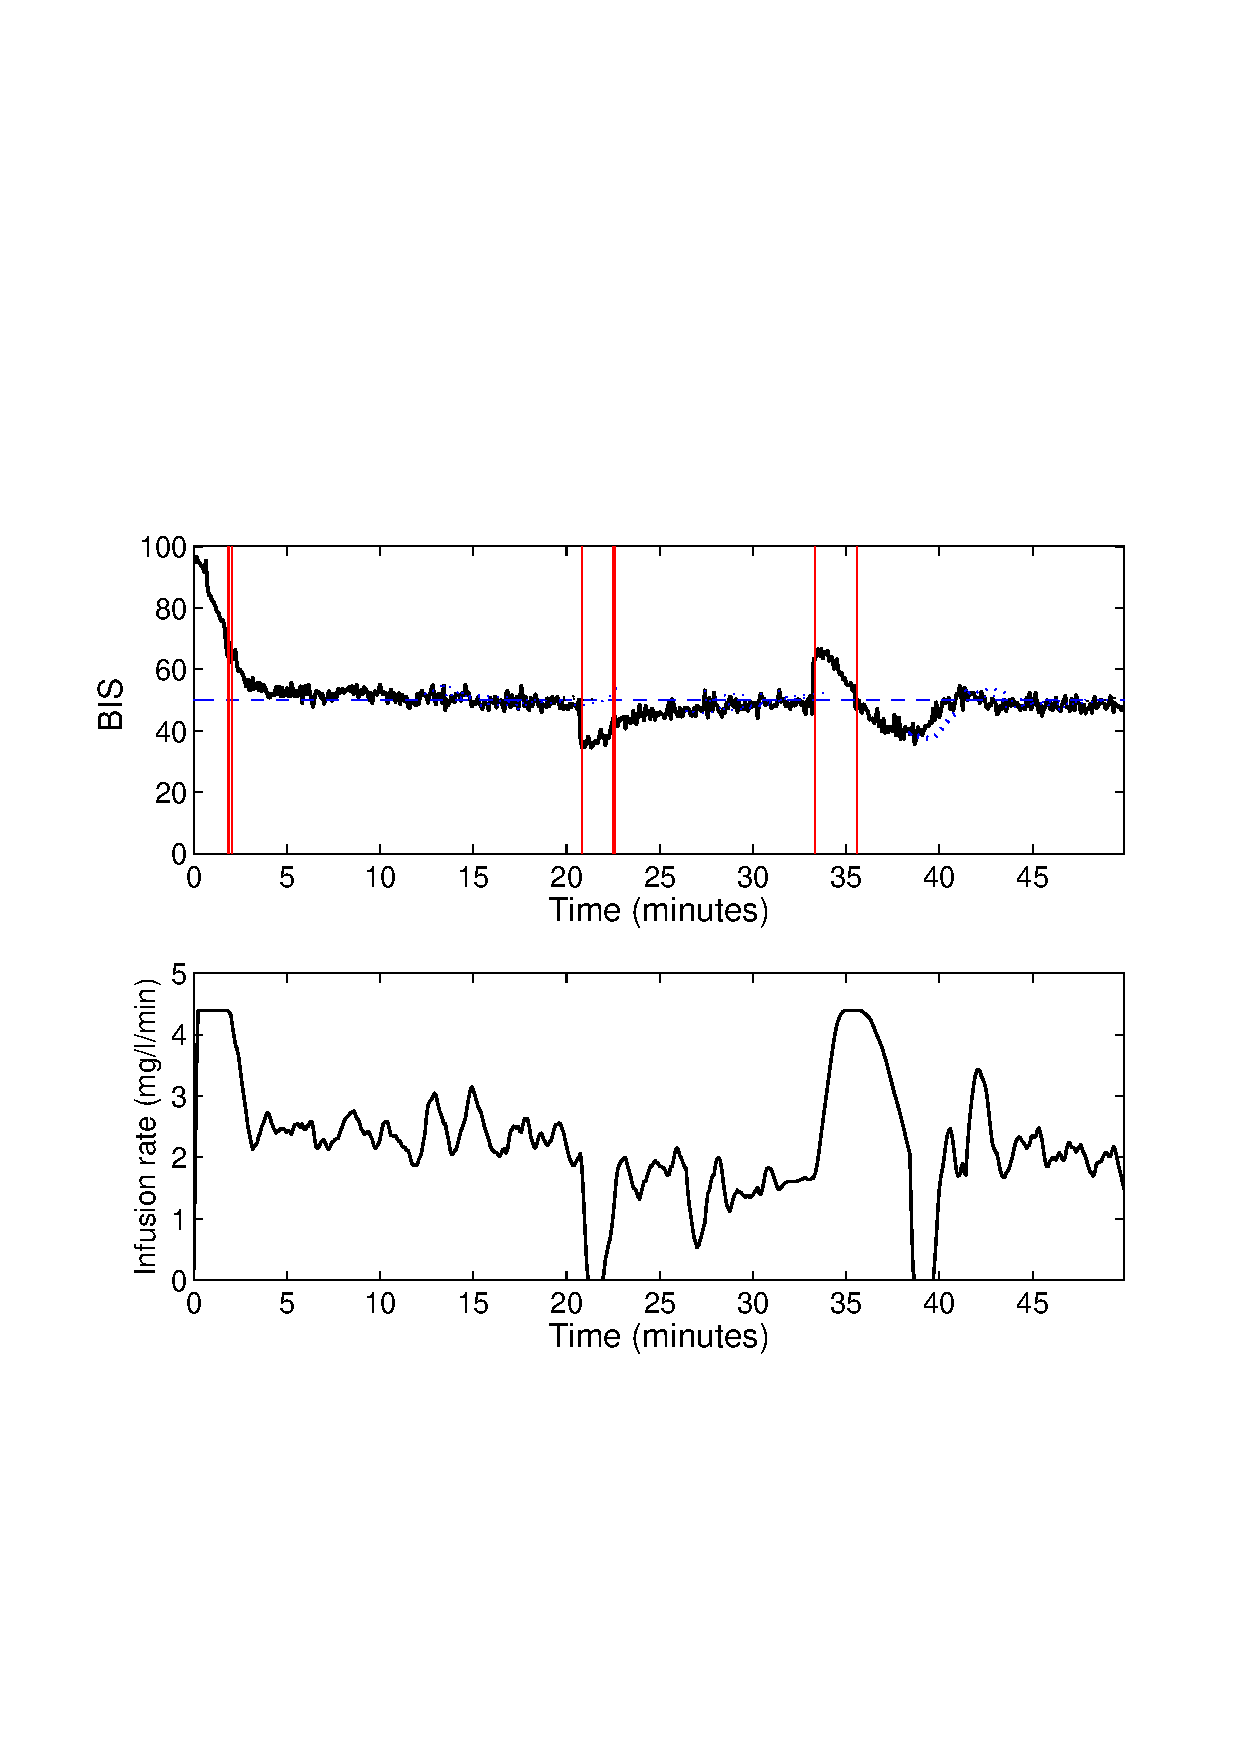
\includegraphics[width=0.40\textwidth]{./pics/aclac_paper/fig2ColsedLoopContrlSim.pdf}%, height=0.45\textwidth
%\caption{Closed-loop control simulation of patient BIS using adaptive predictive control with change detection algorithm. Disturbances appears at $t=20.8 min$ and $t=33.3 min$. Upper figure show BIS evolution (solid line), BIS target (dashed line) and model predictions (dotted line). Vertical lines indicates a change detection. Lower figure presents infusion rate.}
\caption{ACLAC simulation result. Disturbances appears at $t = 20.8$ min and $t = 33.3$ min. The upper figure shows BIS evolution (solid line), BIS target (dashed line) and model predictions (dotted line). Vertical lines indicate detected change points. The lower figure presents the infusion rate.}
\label{fig:fig2ColsedLoopContrlSim}
\end{figure}

Figure~\ref{fig:fig1Comparison} shows a comparison of the proposed
ACLAC performance is done with a similar algorithm without change
detection. Change detection is shown with vertical lines. We can see
that if there are no disturbance both approaches show identical
performance. However, after the disturbance affects the patient, ACLAC
(solid line) performs better than a similar controller without an
explicit change detection mechanism. The disturbance rejection is
quite effective with ACLAC. Observe that the algorithm without change
detection is not able to take the patient quickly to the target due to
the use of a less accurate model.

\begin{figure}[htb!]
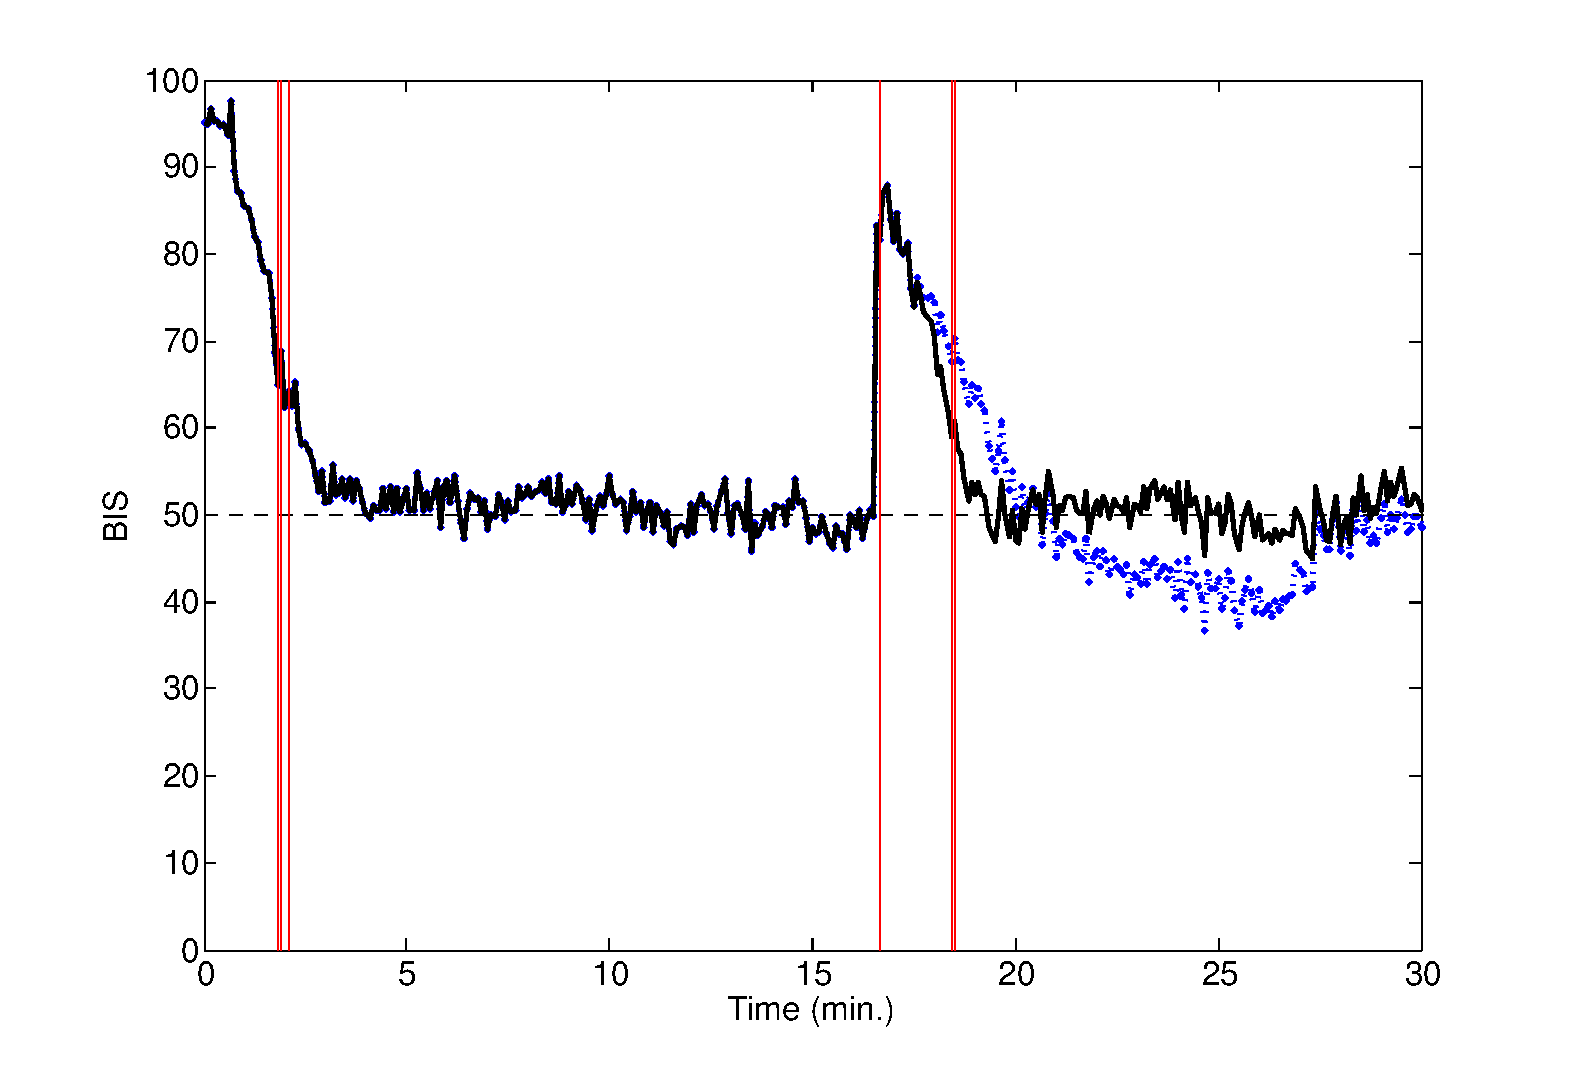
\includegraphics[width=0.45\textwidth]{./pics/aclac_paper/fig1Comparison.pdf}%, height=0.3\textwidth
\caption{Comparison of ACLAC (solid line) and predictive controller
  using a fixed time window for identification (dotted line) instead
  of relying on explicit change detection.}
\label{fig:fig1Comparison}
\end{figure}

\section{Conclusion and future work}
Close-loop control of hypnosis for patients undergoing general
anesthesia is an important problem that is challenging because of the
inter- and intra-patient variability in response behavior.  We
proposed ACLAC - an adaptive scheme of the controller that uses
explicit change detection mechanism for quicker adaptation to the
changes in patients response.

We performed experimental evaluation of the change detection mechanism
on real data collected from the patients and of ACLAC as a whole in
the simulation.  The results indicate that introduced explicit change
detection mechanism indeed improves the performance of ACLAC in
comparison with analogous adaptive schemes based on fixed time window
instead of detecting changes.

In our future work we plan to (1)~perform more extensive evaluation of
the considered change detection method with other relevant approaches
including e.g. PHT-FM~\cite{GamaRealTimeAlg}, CUSUM~\cite{Cusum}, ADWIN~\cite{adwin07} and Quantile Index~\cite{Maslov_QI} on a larger set of BIS signals, and 
(2)~validating the proposed closed-loop hypnosis control approach in
the real operational settings, i.e. in a surgery room.
%
%Our approach is unsupervised but also have limitations which are described above.
%
%We believe that the best approach is to use ensemble method which incorporates strong points from other methods.
%
%In a future work we want to modify proposed approach to more consistent for on-line sequential processing and change detection.
% We want to modify optimal partitioning method for on-line usage and
% use it in ensemble with sequential on-line change detection methods
% (PHT-FM, CUSUM, etc.).

%\section{Acknowledgements}
\paragraph{Acknowledgements.}
This work is under the auspicious of the research Project
DPI2010-18278 supported by ``Ministerio de Ciencia e Innovación" of the
Spanish Government.

%~\cite{GamaRealTimeAlg}
%~\cite{GamaDecisionSupportSystems}

%\bibliographystyle{latex8}
%\bibliographystyle{abbrv}
\bibliography{references_aclac}

